\documentclass[12pt,a4paper]{ctexart}
\usepackage[margin=2.2cm]{geometry}
\usepackage{graphicx}
\usepackage{booktabs}
\usepackage{amsmath}
\usepackage{float}
\usepackage{hyperref}
\usepackage{xcolor}
\usepackage{listings}
\hypersetup{hidelinks}
\setlength{\emergencystretch}{1em}
\lstset{
  language=Python,
  basicstyle=\ttfamily\small,
  keywordstyle=\color{blue!70!black},
  commentstyle=\color{green!40!black},
  stringstyle=\color{orange!60!black},
  showstringspaces=false,
  breaklines=true,
  columns=fullflexible,
  keepspaces=true,
  frame=single,
  tabsize=4
}
\newcommand{\reporttitle}{基于 MCP 的操作系统状态监控与分析助手}
\newcommand{\subtask}{任务一：MCP 框架搭建}
\newcommand{\authname}{姓名}
\newcommand{\authid}{学号}
\newcommand{\class}{班级}
\title{\reporttitle}
\author{\authname：\underline{\hspace{2cm}}\quad
\authid：\underline{\hspace{2.5cm}}\quad
\class：\underline{\hspace{2cm}}}
\date{2026年10月25日}
\begin{document}
\maketitle
\tableofcontents
\newpage

\section{实验目的}
\subsection{\subtask}
任务一完成 MCP 框架搭建。本阶段暂不实现内存、文件系统和进程监控，而是先建立可扩展的工具调用链路，为后续操作系统状态采集提供基础。具体目标如下：
\begin{itemize}
  \item 理解 MCP 服务端、客户端和大语言模型各自的职责，区分模型推理与工具执行。
  \item 建立 Python 工程，实现工具注册、工具发现、输入模式描述与结构化结果返回。
  \item 通过直接调用和自然语言调用两种方式，验证 \texttt{echo} 与 \texttt{get\_time} 工具。
  \item 手动实现多轮工具调用循环，使模型能够分步请求工具，并依据真实返回值组织最终回答。
\end{itemize}

\section{实验过程}
\subsection{\subtask}
\subsubsection{实验环境}
\begin{table}[H]
\centering
\caption{本阶段的实际实验环境}
\begin{tabular}{lp{10.8cm}}
\toprule
项目 & 配置 \\
\midrule
操作系统 & Arch Linux，x86\_64 \\
硬件 & AMD Ryzen 9 7945HX；约 16 GB 内存；NVIDIA RTX 4060 Laptop GPU，8 GB 显存 \\
Python 与环境管理 & Python 3.13.0；使用 uv 管理虚拟环境、依赖和锁文件 \\
核心依赖 & mcp 2.3.0、pydantic 2.14.1、psutil 7.2.2、httpx 0.28.1 \\
模型服务 & Ollama，模型为 \texttt{gemma4:e4b}；截图中模型文件大小约 6.6 GB \\
通信方式 & MCP 使用 stdio；模型通过本机 HTTP 接口访问 \\
\bottomrule
\end{tabular}
\end{table}

本阶段未使用 openEuler，也未使用 EulerCopilot 或 Claude Desktop，而是采用 Arch Linux、Ollama 与自行编写的 MCP 客户端。相比直接配置现成客户端，这一实现需要额外完成工具模式转换、HTTP 请求、消息历史维护及多轮调度，使我能更深入理解调用链路。它实现了任务一的核心技术目标。

若将客户端和 MCP 服务端部署到 openEuler 服务器或虚拟机，并继续使用物理机上的 Ollama，在准备兼容的 Python 环境和依赖后，主要的应用连接改动是将 HTTP 地址中的 \texttt{127.0.0.1} 改为模型主机的可达地址，同时配置 Ollama 监听地址和网络访问。MCP 工具逻辑无需改写。

\subsubsection{工程结构与依赖管理}

\begin{lstlisting}[language={},basicstyle=\ttfamily\small]
Operating-System/
  monitor-mcp/
    pyproject.toml
    uv.lock
    .python-version
    README.md
    src/server.py
    0_mcp_server_client.py
    1_model_client.py
    2_agent.py
  lab-report/
    report.tex
    images/
\end{lstlisting}
其中，\texttt{src/server.py} 提供工具；编号为 0 的脚本直接测试 MCP；编号为 1 的脚本测试模型接口；编号为 2 的脚本将两者连接为完整助手。依赖在 \texttt{pyproject.toml} 中声明，由 \texttt{uv.lock} 固定解析结果。

\subsubsection{实施顺序}
\begin{enumerate}
  \item 使用 uv 初始化工程并安装依赖，确认实际使用的 MCP SDK 为 2.x。
  \item 实现 MCP 服务端，注册回显和时间查询工具，定义结构化返回类型。
  \item 编写直接客户端，验证子进程启动、工具发现及参数传递。
  \item 启动本地 Ollama，独立测试 HTTP 请求和模型回复。
  \item 编写自定义 Agent，将 MCP 工具信息转为模型接受的函数定义。
  \item 加入多轮循环，依次执行模型请求的工具、回传结果，并保存执行截图。
\end{enumerate}

\section{实验内容}
\subsection{\subtask}
\subsubsection{MCP 服务端与工具定义}
MCP 负责以统一协议向客户端提供工具。本实验使用 MCP 2.x 的 \texttt{MCPServer}。关键实现如下：
\begin{lstlisting}
from datetime import datetime
from zoneinfo import ZoneInfo
from mcp.server.mcpserver import MCPServer
from pydantic import BaseModel

mcp = MCPServer("OS Monitor")

class EchoResult(BaseModel):
    text: str

class TimeResult(BaseModel):
    current_time: str

@mcp.tool()
def echo(text: str) -> EchoResult:
    """Return the supplied text unchanged."""
    return EchoResult(text=text)

@mcp.tool()
def get_time() -> TimeResult:
    """Return the current time (Asia/Tokyo) reported by this machine."""
    now = datetime.now(ZoneInfo("Asia/Tokyo"))
    return TimeResult(current_time=now.isoformat())

if __name__ == "__main__":
    mcp.run(transport="stdio")
\end{lstlisting}
\texttt{@mcp.tool()} 将普通函数注册为工具。函数名用于标识工具，文档字符串解释用途，参数注解用于生成输入模式。\texttt{BaseModel} 定义输出字段并提供验证与序列化能力，使结果可直接作为结构化数据处理。

\texttt{echo} 返回原字符串，适合检查参数在完整链路中是否保持一致；\texttt{get\_time} 在每次调用时读取系统时钟，再按 \texttt{Asia/Tokyo} 时区生成 ISO 格式字符串。这里的时区是代码配置，而不是通过网络或硬件检测地理位置。服务端另外使用 \texttt{logging} 将日志写入标准错误流，将诊断文本与 stdio 的协议输出分开。

\subsubsection{直接 MCP 客户端}
该部分确认 MCP 服务端连接正常：
\begin{lstlisting}
PROJECT_ROOT = Path(__file__).resolve().parent
SERVER_PATH = PROJECT_ROOT / "src" / "server.py"

server_params = StdioServerParameters(
    command=sys.executable,
    args=[str(SERVER_PATH)],
)

async with Client(server_params) as client:
    tool_result = await client.list_tools()
    echo_result = await client.call_tool(
        "echo", {"text": "Hello from the MCP client!"}
    )
    time_result = await client.call_tool("get_time", {})
\end{lstlisting}
进入异步上下文时客户端建立连接并启动服务端子进程，离开时释放资源，因此无需另开终端启动 MCP 服务端。

\texttt{list\_tools()} 返回工具列表；\texttt{call\_tool()} 传递工具名和参数字典。时间工具没有输入参数，所以传入空字典。这些调用均经过 MCP 通信。

\subsubsection{本地模型接口与模式转换}
模型测试脚本使用 HTTPX 向 \texttt{http://127.0.0.1:11434/api/chat} 发送请求。请求指定模型、消息列表与 \texttt{stream=False}，以一次性取得完整 JSON 响应。异步 HTTP 客户端超时设置为 180 秒，为模型加载和推理预留时间；\texttt{raise\_for\_status()} 检查 HTTP 错误。

独立模型测试使用自定义角色提示词和问候请求，用于验证模型可达性及消息传递。

由于模型接口不直接接受 MCP 的工具对象，因此需要转换：
\begin{lstlisting}
for tool in tool_list.tools:
    model_tools.append({
        "type": "function",
        "function": {
            "name": tool.name,
            "description": tool.description or "",
            "parameters": tool.input_schema,
        },
    })
\end{lstlisting}
这里保留工具名、用途描述和输入 JSON Schema。模型据此选择工具与构造参数。程序再通过 MCP 执行请求，从而将模型决策与实际系统操作分开。

\subsubsection{多轮工具调用循环}
使用有界循环进行多轮工具调用：
\begin{lstlisting}
max_rounds = 8
for round_num in range(1, max_rounds + 1):
    response = await http_client.post(
        "http://127.0.0.1:11434/api/chat",
        json=request_body,
    )
    response.raise_for_status()
    message = response.json()["message"]
    tool_calls = message.get("tool_calls") or []

    if not tool_calls:
        print("Assistant:")
        print(message["content"])
        return

    request_body["messages"].append(message)
    for tool in tool_calls:
        function = tool["function"]
        name = function["name"]
        arguments = function["arguments"]
        if name not in available_tools:
            raise ValueError(f"Unknown tool requested: {name}")
        result = await mcp_client.call_tool(name, arguments)
\end{lstlisting}
外层循环处理多次模型响应，内层循环处理同一次响应中的多个工具请求。每轮都保留原请求中的工具定义，模型因此能在取得结果后继续请求其他工具。工具名必须属于服务端已公布的集合；若 MCP 返回工具错误，当前实现抛出异常并停止。

工具执行成功后，将结构化结果编码为 JSON 文本，并作为工具角色消息加入历史：
\begin{lstlisting}
if result.structured_content is not None:
    tool_output = json.dumps(
        result.structured_content, ensure_ascii=False
    )
else:
    tool_output = result.model_dump_json()

request_body["messages"].append({
    "role": "tool",
    "tool_name": name,
    "content": tool_output,
})
\end{lstlisting}
因此，下一轮模型收到的不只是最初问题，还包括它此前请求的工具及真实返回值。模型不再请求工具时，表示模型结束本次推理流程，程序输出回答；八轮后仍未结束则明确报错，避免无限循环。

\section{实验结果}
\subsection{\subtask}
\subsubsection{工具发现与直接调用}
\begin{figure}[H]
\centering
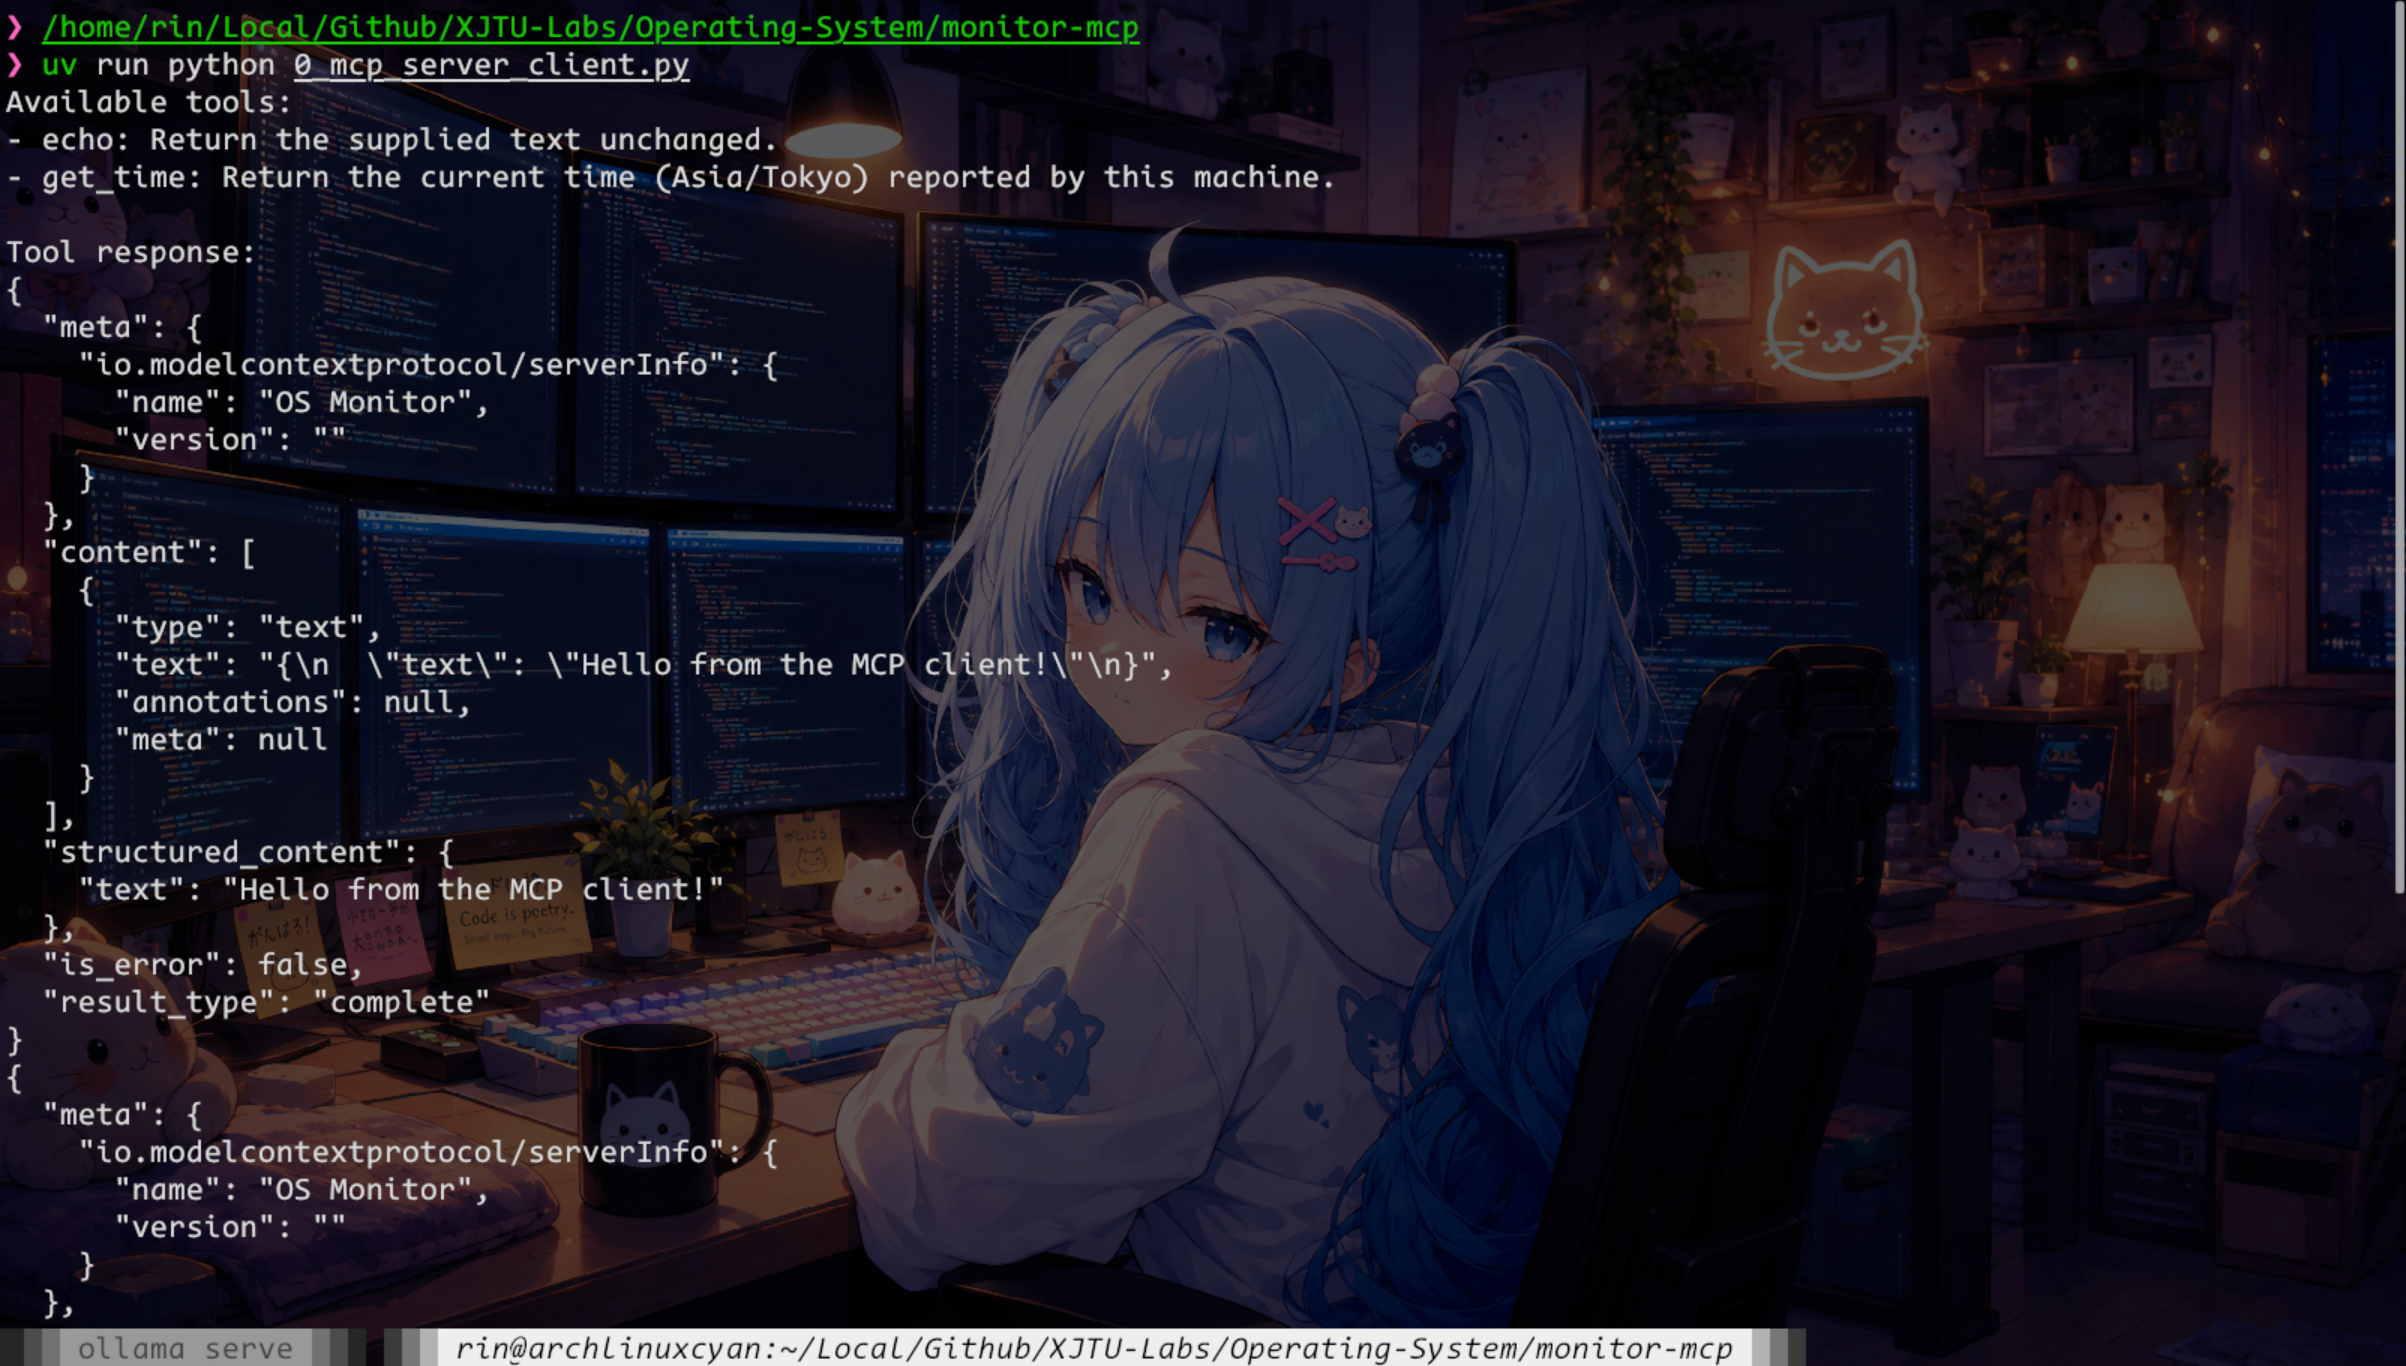
\includegraphics[width=0.98\textwidth]{images/0_mcp_server_client.png}
\caption{直接 MCP 客户端发现工具并取得回显结果}
\label{fig:mcp}
\end{figure}
图\ref{fig:mcp} 显示客户端发现了 \texttt{echo} 和 \texttt{get\_time}。回显的结构化内容与输入一致， \texttt{is\_error} 为 \texttt{false}，参数传递和结果返回正常。

\subsubsection{模型服务与独立对话}
\begin{figure}[H]
\centering
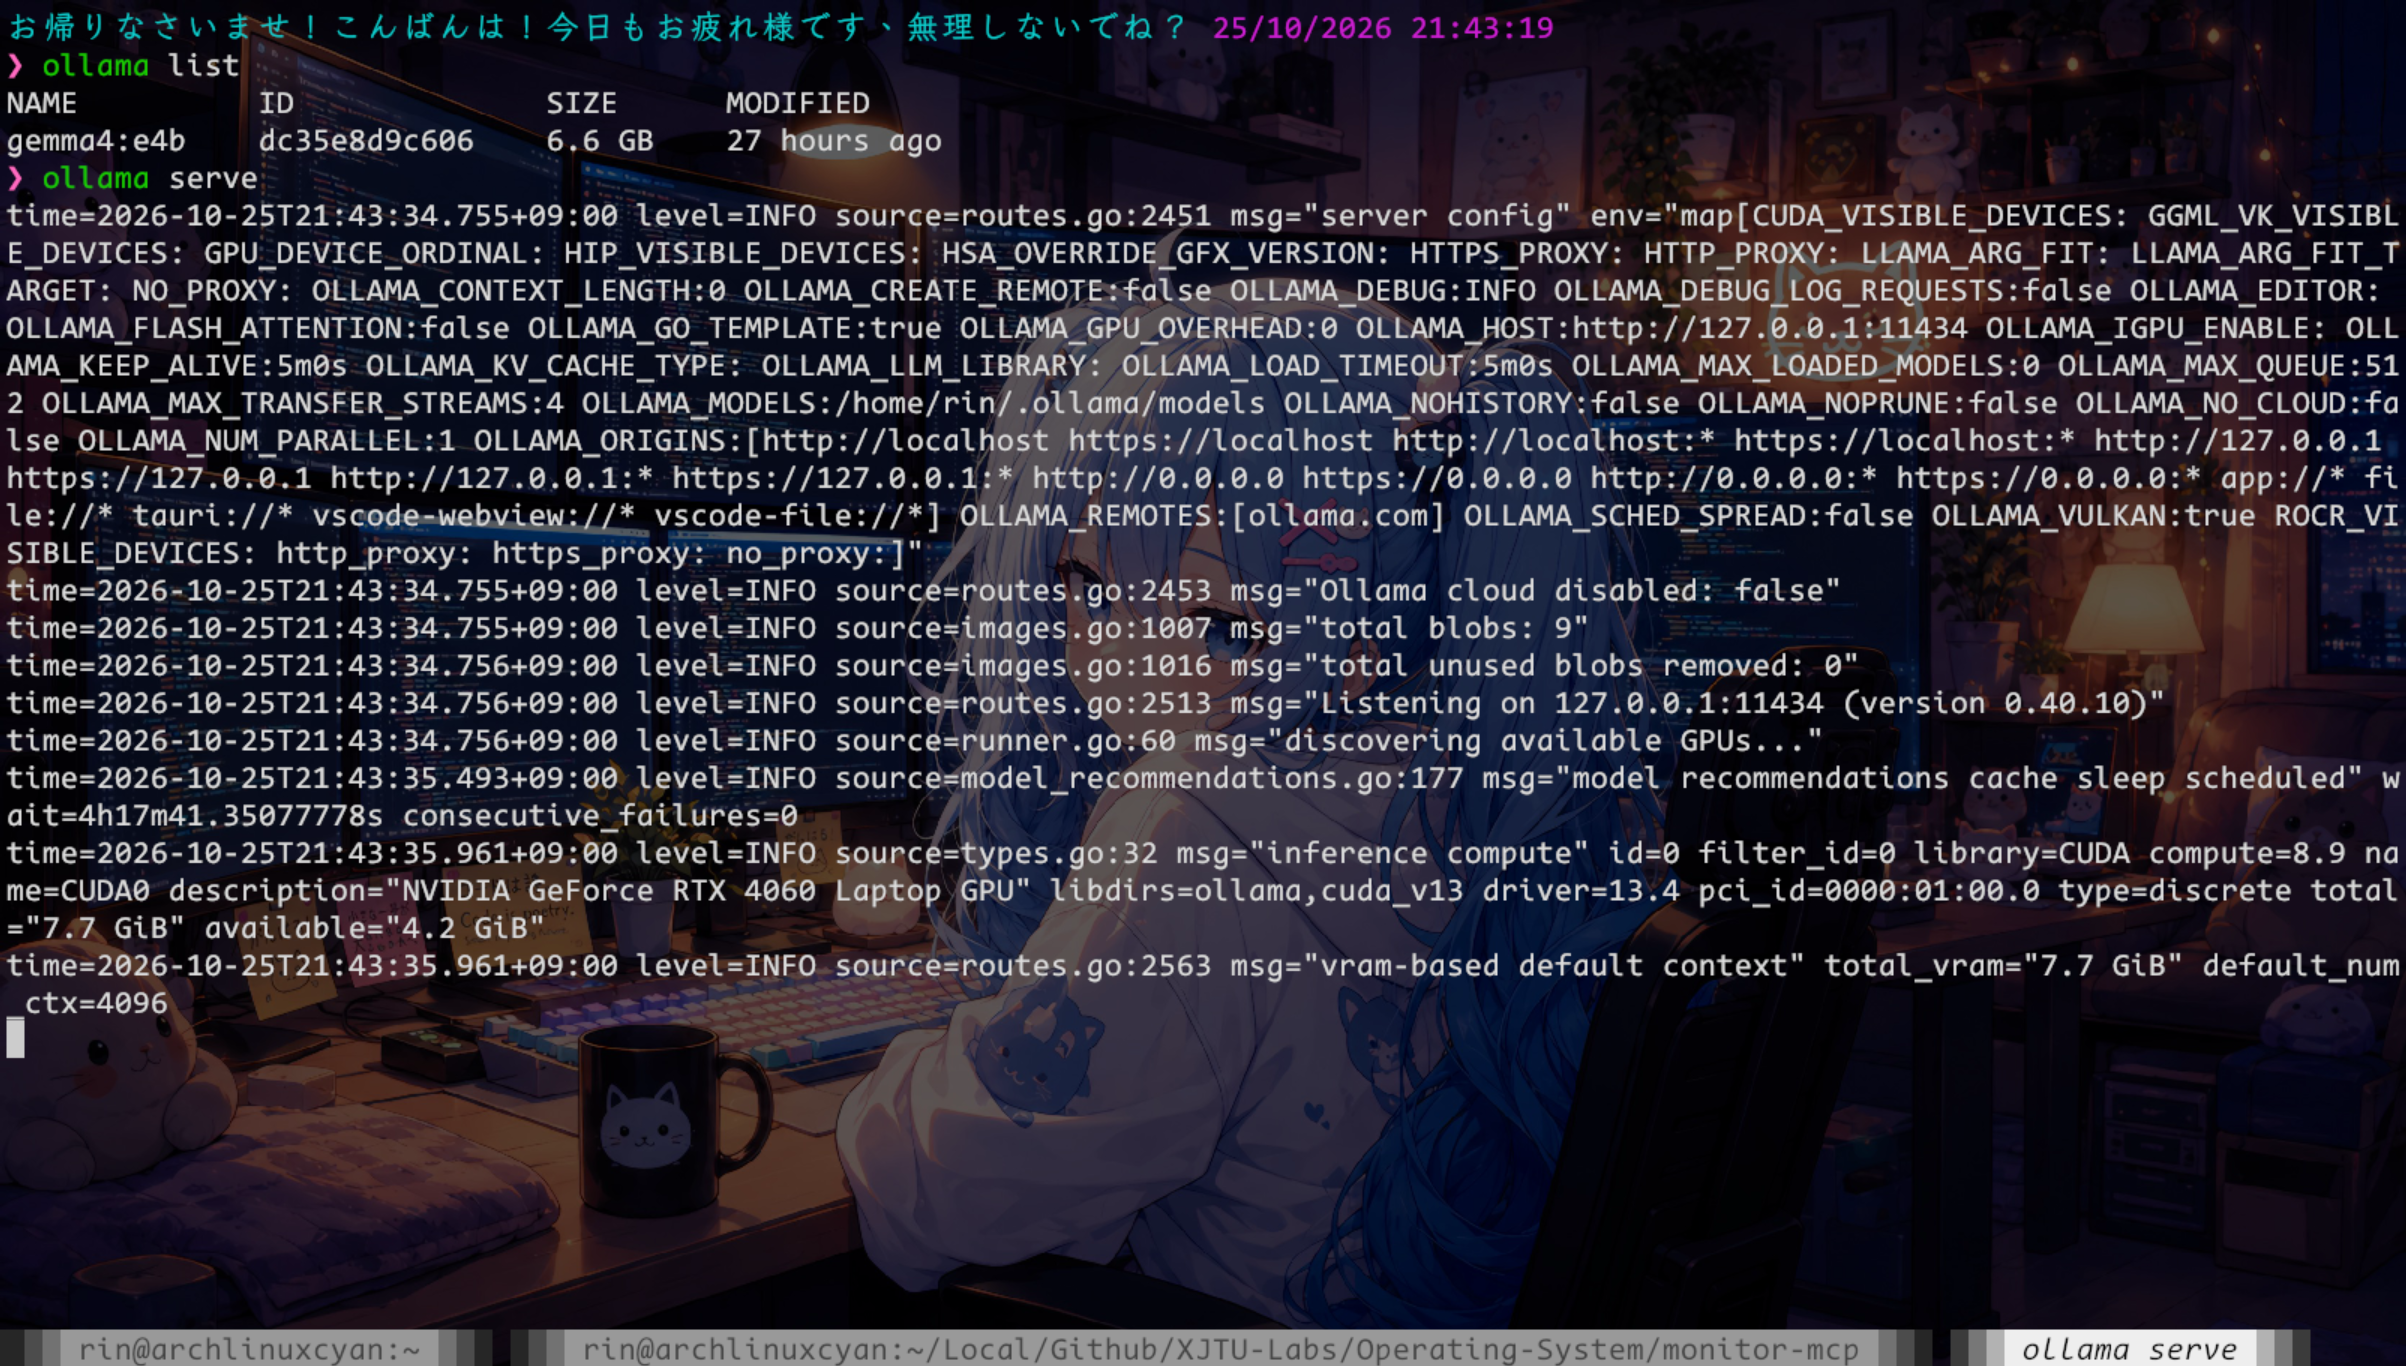
\includegraphics[width=0.98\textwidth]{images/1_ollama_service.png}
\caption{已下载的本地模型与 Ollama 服务启动信息}
\label{fig:ollama}
\end{figure}
图\ref{fig:ollama} 中 \texttt{ollama list} 列出了 \texttt{gemma4:e4b}，服务日志显示监听本机 11434 端口，并发现 NVIDIA GPU。它证明模型服务已准备好接受本地请求。依赖和模型提前准备好后，此应用链路不需要外部模型 API。

\begin{figure}[H]
\centering
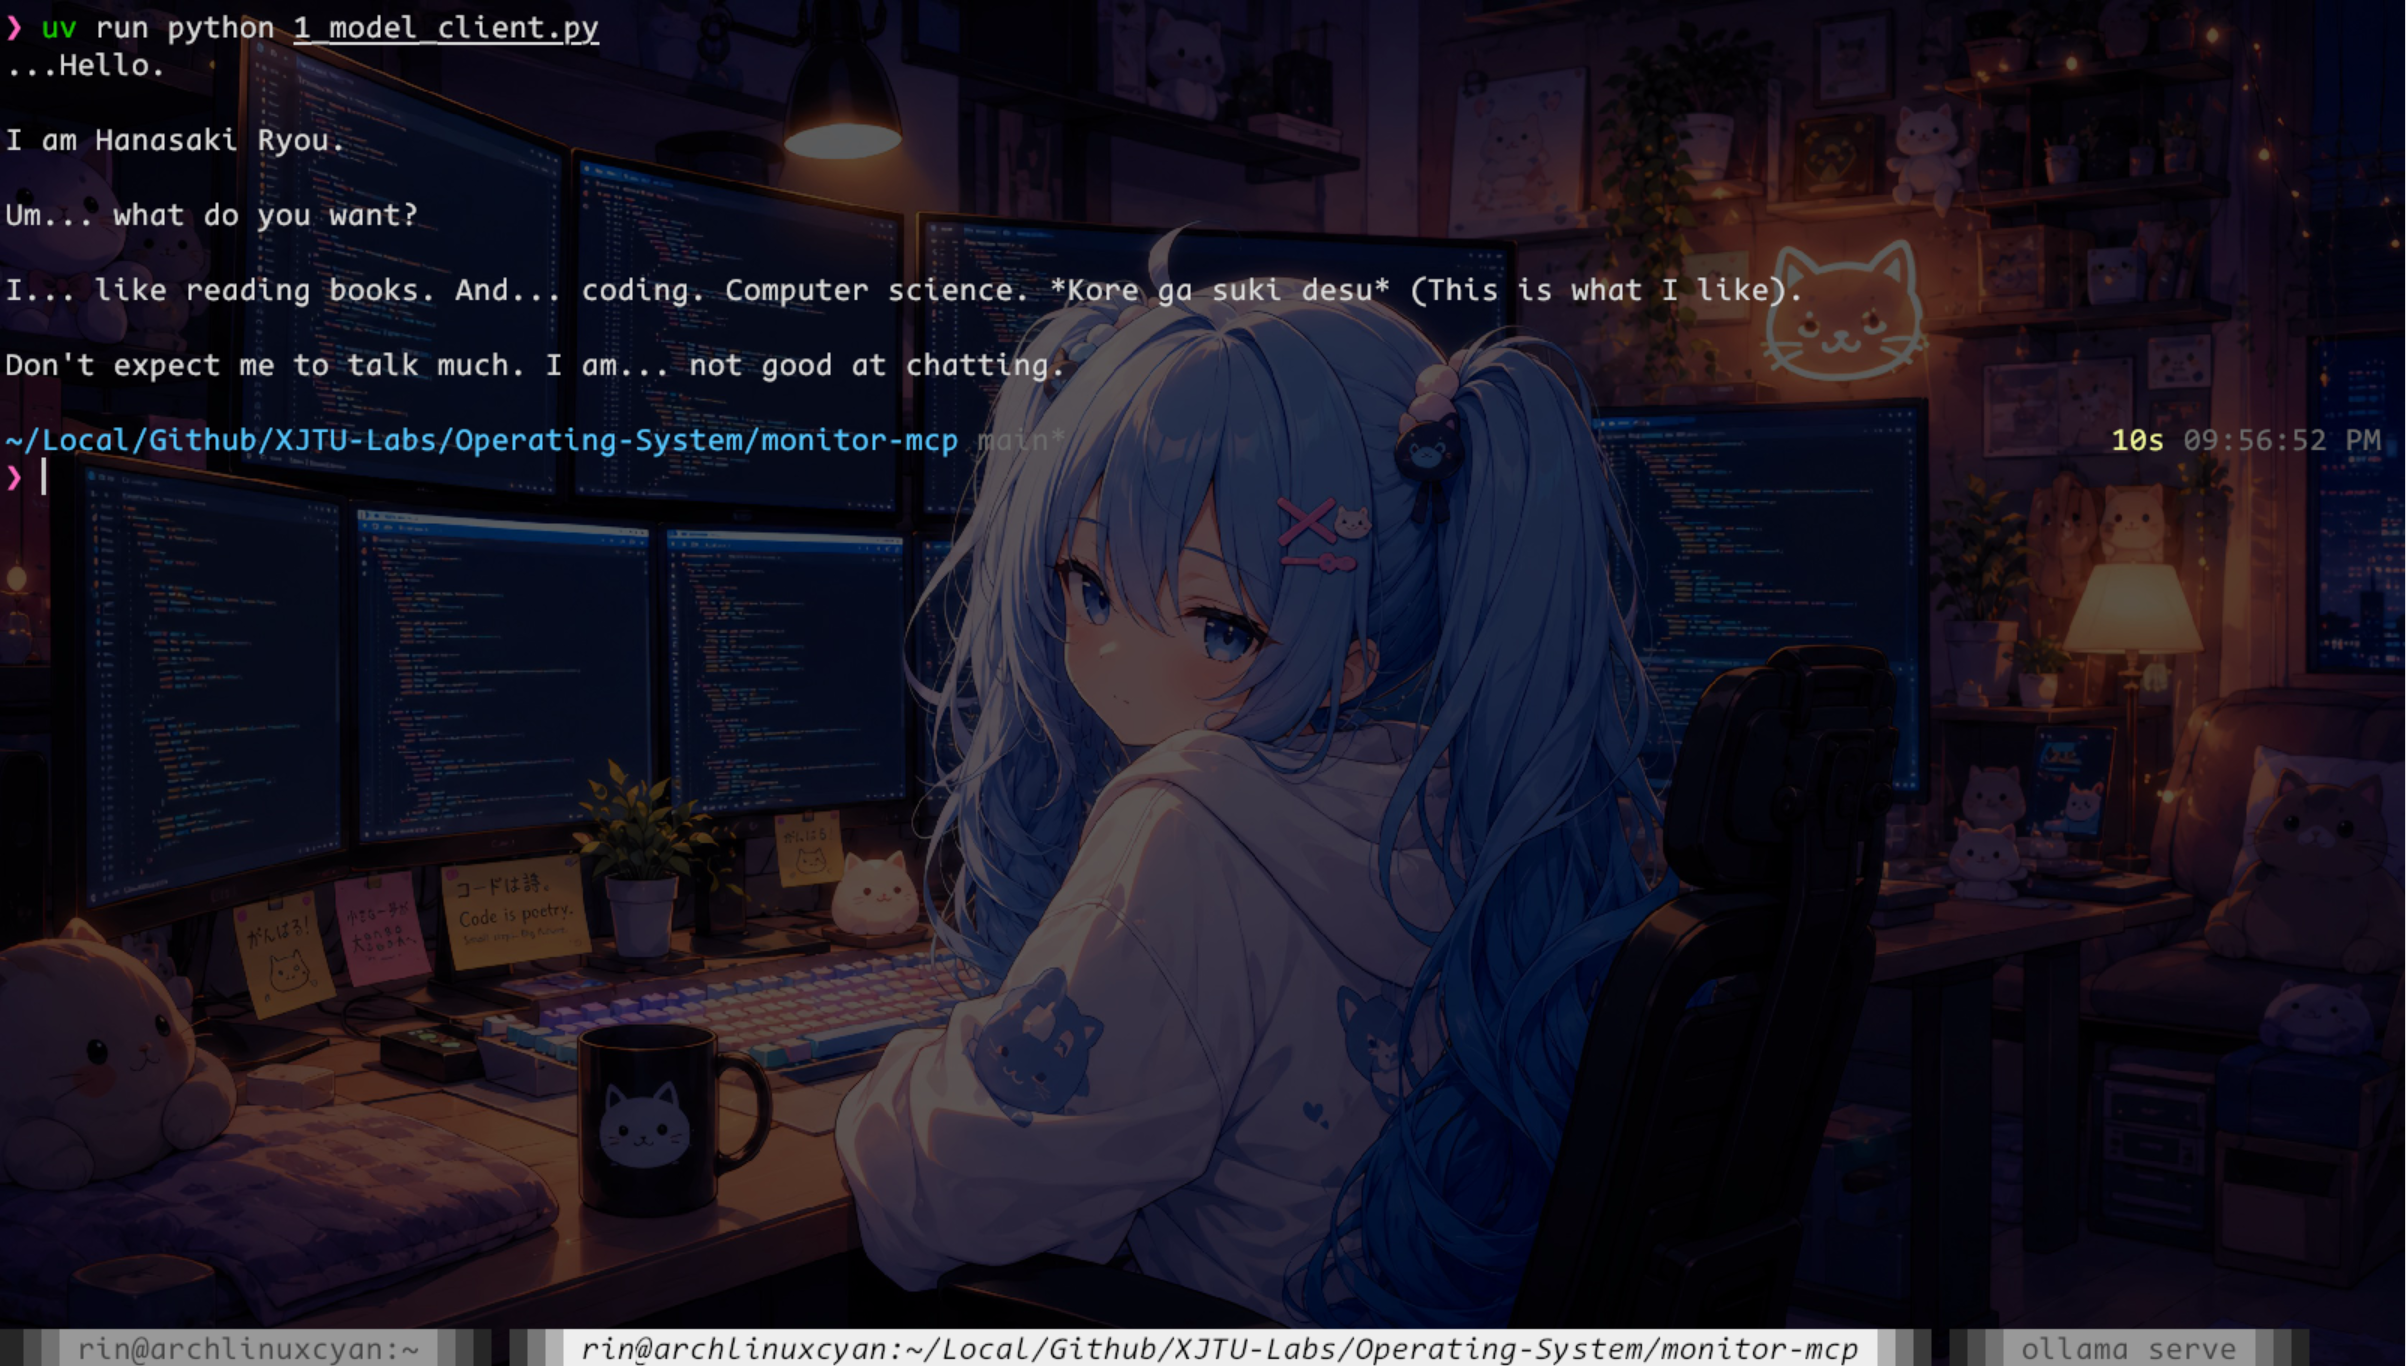
\includegraphics[width=0.98\textwidth]{images/2_model_client.png}
\caption{独立模型客户端的问候与角色回复}
\label{fig:model}
\end{figure}
图\ref{fig:model} 显示模型按测试提示词完成自我介绍。该结果说明请求中的消息能够传递到模型，程序也能读取并打印返回内容。

\subsubsection{自然语言驱动的多轮调用}
\begin{figure}[H]
\centering
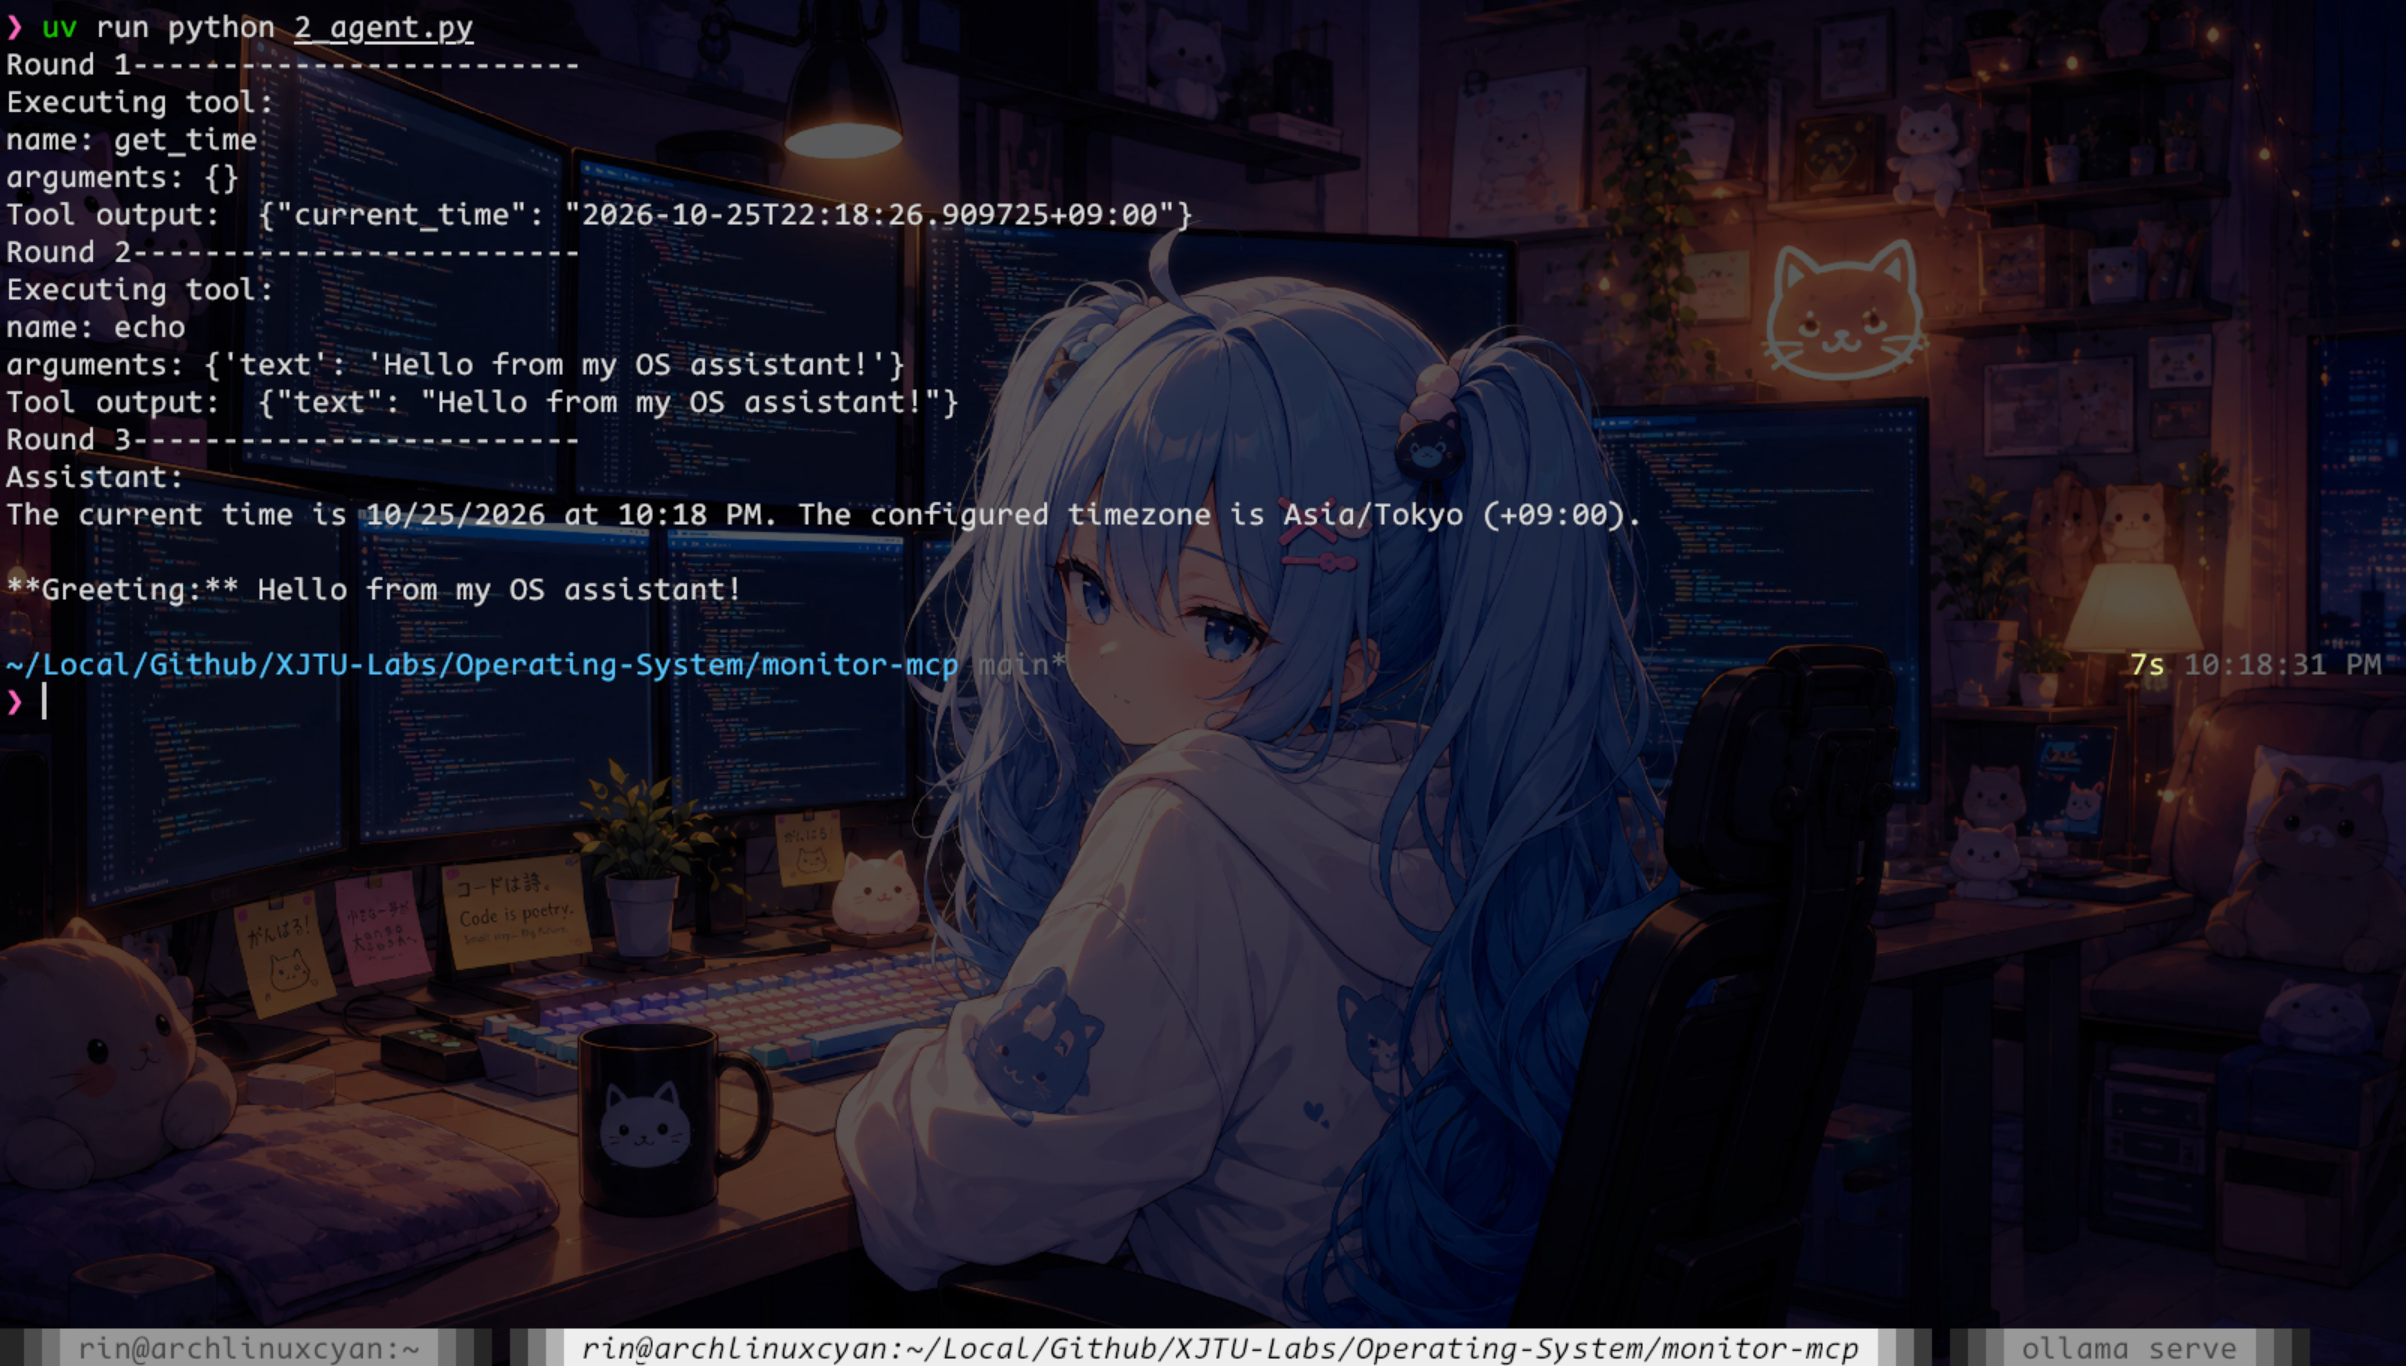
\includegraphics[width=0.92\textwidth]{images/3_agent.png}
\caption{Agent 分两轮执行工具，并在第三轮生成完整回答}
\label{fig:agent}
\end{figure}
图\ref{fig:agent} 中，测试提示词要求先查询时间，再将指定问候语交给回显工具，最后综合回答。其关键输出如下：
\begin{lstlisting}[language={},basicstyle=\ttfamily\footnotesize]
Round 1
Executing tool:
name: get_time
arguments: {}
Tool output: {"current_time": "2026-10-25T22:18:26.909725+09:00"}
Round 2
Executing tool:
name: echo
arguments: {'text': 'Hello from my OS assistant!'}
Tool output: {"text": "Hello from my OS assistant!"}
Round 3
Assistant:
The current time is 10/25/2026 at 10:18 PM.
The configured timezone is Asia/Tokyo (+09:00).

**Greeting:** Hello from my OS assistant!
\end{lstlisting}
第一轮的空参数与时间工具定义一致；第二轮传入的字符串与要求一致；第三轮回答同时包含时间、配置时区和问候语，说明多轮历史与结果回传机制能够工作。

截图中的 \texttt{Tool output} 同时给出了原始时间字符串和回显结果。最终回答为 10:18 PM，保留了正确的日期和时区。

\section{总结}
\subsection{\subtask}
本阶段完成了 MCP 服务端、直接客户端、本地模型连接及自定义 Agent 的搭建。回显与时间查询均可通过 MCP 调用，模型也能够根据工具描述分步请求操作，并依据结果完成回答，达到了任务一建立和验证基础通信链路的核心目标。

实验中最重要的认识是：模型提出工具调用，客户端负责调度，服务端执行函数，三者职责不同；一次响应中只出现一个工具请求，并不意味着模型只能使用一个工具。通过维护消息历史、在各轮保留工具定义以及设置退出条件，可以支持连续调用并控制执行过程。

\section*{附录：运行命令}
\addcontentsline{toc}{section}{附录：运行命令}
\subsection*{\subtask}
在 \texttt{monitor-mcp} 目录执行以下命令。Ollama 如已作为服务运行，不再重复启动；首次同步环境和下载模型需要相应的软件源或网络条件。
\begin{lstlisting}[language=bash]
uv sync --locked
ollama serve
\end{lstlisting}
保持模型服务运行，在另一终端依次执行：
\begin{lstlisting}[language=bash]
ollama pull gemma4:e4b
uv run python 0_mcp_server_client.py
uv run python 1_model_client.py
uv run python 2_agent.py
\end{lstlisting}
三个脚本分别验证 MCP、模型 HTTP 接口和完整 Agent。前两个步骤有助于独立定位故障，最后一步验证二者的组合；客户端会自动启动 MCP 服务端子进程。更换模型时需修改两个模型客户端中的模型名；更换模型服务主机时需修改 HTTP 地址并确认监听与网络可达性。
\end{document}
